\iffalse
\let\negmedspace\undefined
\let\negthickspace\undefined
\documentclass[journal,12pt,twocolumn]{IEEEtran}
\usepackage{cite}
\usepackage{amsmath,amssymb,amsfonts,amsthm}
\usepackage{algorithmic}
\usepackage{graphicx}
\usepackage{textcomp}
\usepackage{xcolor}
\usepackage{txfonts}
\usepackage{listings}
\usepackage{enumitem}
\usepackage{mathtools}
\usepackage{gensymb}
\usepackage{comment}
\usepackage[breaklinks=true]{hyperref}
\usepackage{tkz-euclide}
\usepackage{listings}
\usepackage{gvv}
\def\inputGnumericTable{}
\usepackage[latin1]{inputenc}
\usepackage{color}
\usepackage{array}
\usepackage{longtable}
\usepackage{calc}
\usepackage{multirow}
\usepackage{hhline}
\usepackage{ifthen}
\usepackage{lscape}

\newtheorem{theorem}{Theorem}[section]
\newtheorem{problem}{Problem}
\newtheorem{proposition}{Proposition}[section]
\newtheorem{lemma}{Lemma}[section]
\newtheorem{corollary}[theorem]{Corollary}
\newtheorem{example}{Example}[section]
\newtheorem{definition}[problem]{Definition}
\newcommand{\BEQA}{\begin{eqnarray}}
\newcommand{\EEQA}{\end{eqnarray}}
\newcommand{\define}{\stackrel{\triangle}{=}}
\theoremstyle{remark}
\newtheorem{rem}{Remark}
\begin{document}

\bibliographystyle{IEEEtran}
\vspace{3cm}

\title{GATE -BM 16}
\author{EE23BTECH11057 - Shakunaveti Sai Sri Ram Varun$^{}$% &lt;-this % stops a space
}
\maketitle
\newpage
\bigskip
\vspace{2cm}
\textbf{Question: }
For the circuit given below, choose the angular frequency $ \omega_0$ at which voltage across capacitor has maximum amplitude?
\begin{figure}[h!]
    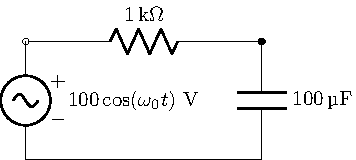
\includegraphics[width = \columnwidth]{2023/BM/16/figs/c_fig1.pdf}
    \caption{circuit }
    \centering
    \label{fig: bm_16_fig_1}
\end{figure}\\
\begin{enumerate}
    \item[(A)] 1000\\
    \item[(B)] 100\\
    \item[(C)] 1\\
    \item[(D)] 0   
\end{enumerate}
\hfill(GATE BM 2023 question 16)\\
\textbf{Solution}:\\
\fi
\begin{table}[h!] 
\centering
\begin{tabular}{|c|c|c|}
    \hline
    \textbf{Parameter} & \textbf{Description} & \textbf{Value} \\
    \hline
    $V_i(j\omega)$ & Input voltage & $100$ \\
    \hline
    $v_c(t)$ & Potential difference across Capacitor & ? \\
    \hline
    $V_c(s)$ & Potential difference across Capacitor & $V_c(s)$ \\
    \hline
    $H(s)$ & Transfer function & $\frac{V_c(s)}{V_i(s)}$ \\
    \hline
    $V_o$ & Amplitude of input voltage & $100 \, \text{V}$ \\
    \hline
    $R$ & Resistance in circuit & $1 \, \text{k}\Omega$ \\
    \hline
    $C$ & Capacitance in circuit & $100 \, \mu\text{F}$ \\
    \hline
    $\omega_o$ & Angular frequency of input voltage & $\omega_o$ \\
    \hline
\end{tabular}


\caption{input values}
\label{tab: table-bm16}
\end{table}

\begin{align}
V_c\brak{s}&= \frac{V_1\brak{s}\frac{1}{sC}}{R+\frac{1}{sC}}\\
\implies H\brak{s} &= \frac{1}{1+ sRC}\\
\implies H\brak{j\omega} &= \frac{1}{1+j\omega RC}\\
|H\brak{j\omega}| &= \frac{1}{\sqrt{1+\brak{\omega RC}^2}}
\end{align}
\begin{figure}[h!]
    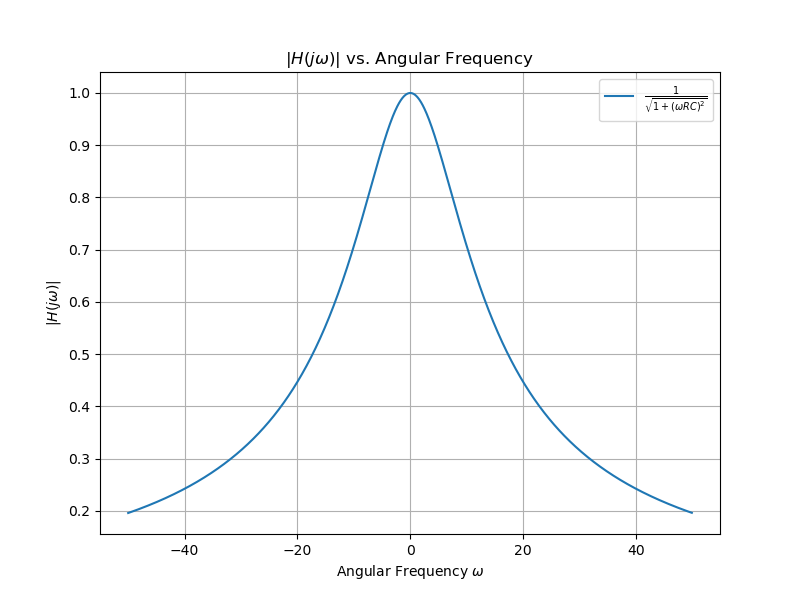
\includegraphics[width = \columnwidth]{2023/BM/16/figs/Figure_1.png}
    \caption{$ |H\brak{j\omega}|$ }
    \centering
    \label{fig: bm_16_fig_2}
\end{figure}


\begin{figure}[h!]
    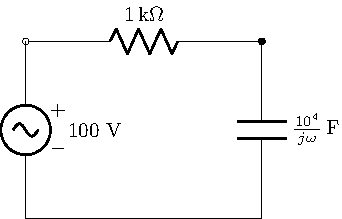
\includegraphics[width = \columnwidth]{2023/BM/16/figs/c_fig2.pdf}
    \caption{circuit in $ \omega$-domain }
    \centering
    \label{fig: bm_16_fig_3}
\end{figure}

\begin{align}
v_c\brak{t}&= \frac{100}{\sqrt{1+\brak{\omega_o RC}^2}}\brak{\cos{\omega_o t + \arctan\brak{\frac{1}{\omega_o RC}}}}
\end{align}
Maximum amplitude of $ v_c\brak{t}$ occurs at $ \omega_o=0$
\begin{align}
\therefore \omega_o =0
\end{align}
$ \therefore$ maximum value of $ v_c\brak{t}$ at steady state is $ 100$ Volts.
